\documentclass[tikz]{standalone}
\begin{document}

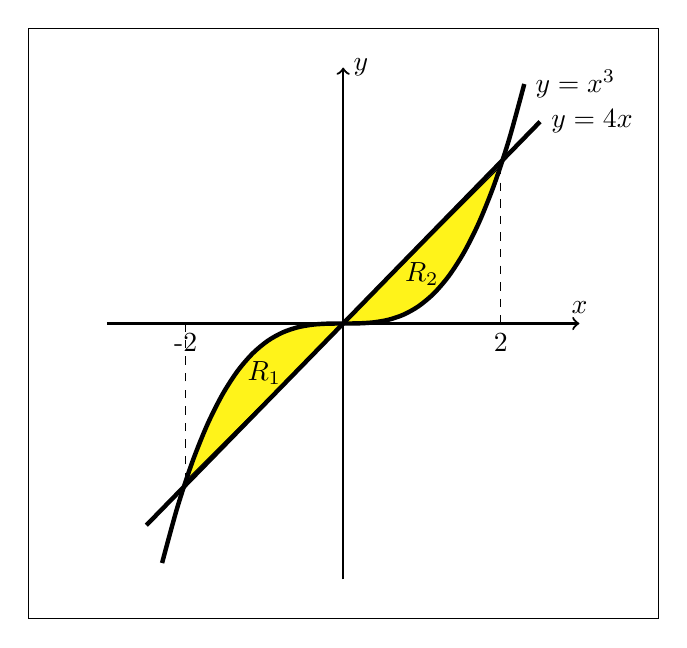
\begin{tikzpicture}[yscale=0.25]
  \draw[fill=white] (-4,-15) rectangle ++(8,30);

  % draw axes
  \draw[thick,->] (-3,0) -- (3,0) node[above] {$x$};
  \draw[thick,->] (0,-13) -- (0,13) node[right] {$y$};

  % shade region
  \draw[fill=yellow!90] plot[smooth, samples=100, domain=-2:2] (\x,\x*\x*\x) -- cycle;

  % draw curves
  \draw[ultra thick,domain=-2.3:2.3,smooth,variable=\x,black] plot (\x,\x*\x*\x) node[right] {$y=x^3$};
  \draw[ultra thick,domain=-2.5:2.5,smooth,variable=\x,black] plot (\x,4.1*\x) node[right] {$y=4x$};
      
  \draw[dashed] (2,8) -- (2,0) node[below] {2};
  \draw[dashed] (-2,-8) -- (-2,0) node[below] {-2};

  \draw (-1, -2.5) node {$R_1$};
  \draw (1, 2.5) node {$R_2$};
\end{tikzpicture}
\end{document} 
